%\chapter{Recuperación de información: limInfo} \label{append:limInfo}

\begin{center}
    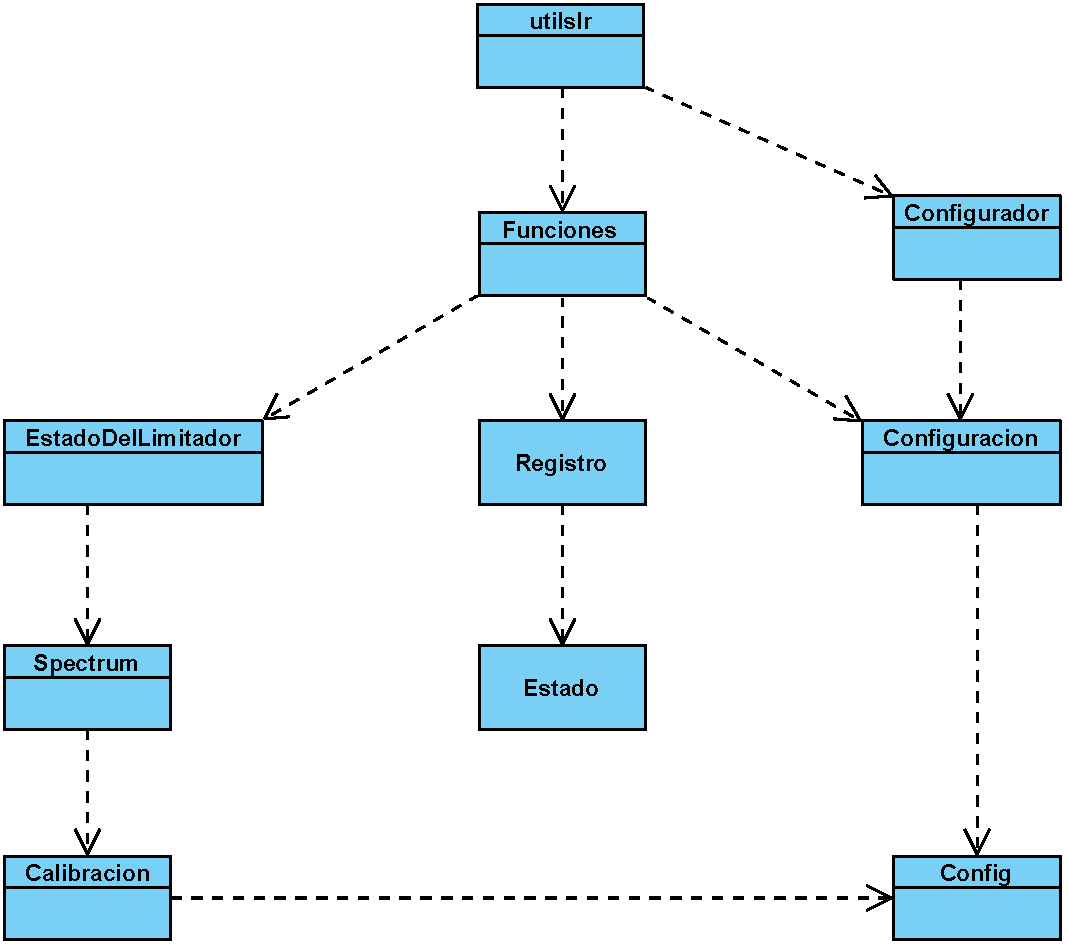
\includegraphics[width=0.9\textwidth]{figuras/lms9-utilslr.pdf}
    \captionof{figure}{Diagrama de dependencias del programa utilslr.}
    \label{fig:utilslr}
\end{center}

El programa \verb|utilslr| recibe serie de comandos como parámetro, principalmente para modificar la configuración del equipo (con \verb|utilslr configura|), pero también para consultar información e incluso generar informes en varios formatos (aunque tras probarlos la mayoría no funcionan).

El programa \verb|utilslr| se usa de forma intensiva en la versión LM7, por parte de la aplicación web. Generalmente se usa para aplicar la configuración y comprobar las contraseñas de usuario.

A continuación se listan los comandos que puede recibir este programa. Aquellos resaltados en negrita representan funcionalidad útil que ha sido exportada al LM11.
\begin{itemize}
	\item clave \$p: comprueba si la contraseña p es correcta.
	\item activaweb \$código \$nSerie \$nDistribuidor: activa la aplicación web.
	\item configuración: devuelve la configuración del equipo, igual que \verb|getConfig|.
	\item \textbf{configura} \$fichero: aplica la configuración definida en el fichero indicado (siempre es \verb|/tmp/conf.tmp|).
	\item \textbraceleft preauth, verifycu\textbraceright: relacionados con verificación de usuarios nuevos. Carecen totalmente de interés para nuestro proyecto.
	\item \textbraceleft sql, xml, yml, json, sqlite\textbraceright  \$fechaIni \$fechaFin \$intervalo: genera volcados en el formato indicado. Solo funcionan sql, xml y json.
	\item \textbraceleft listado, gráfico, actividad\textbraceright: sin usos conocidos.
\end{itemize}